\documentclass[dvipsnames, svgnames, x11names, a4paper, 11pt,]{article}

% URLs and hyperlinks ---------------------------------------
\usepackage{hyperref}
\hypersetup{
    colorlinks=true,
    linkcolor=NavyBlue,
    filecolor=magenta,      
    urlcolor=blue,
}
\usepackage{xurl}
%---------------------------------------------------

\usepackage{graphicx}
\usepackage{listings}
\usepackage{color}
\usepackage{xcolor}

\definecolor{dkgreen}{rgb}{0,0.6,0}
\definecolor{gray}{rgb}{0.5,0.5,0.5}
\definecolor{mauve}{rgb}{0.58,0,0.82}

\lstset{frame=tb,
    language=vhdl,
    aboveskip=3mm,
    belowskip=3mm,
    showstringspaces=false,
    columns=flexible,
    basicstyle=\ttfamily,
    numbers=left,
    numberstyle=\small\color{gray},
    keywordstyle=\bfseries\color{Green4},
    commentstyle=\color{gray},
    stringstyle=\color{mauve},
    breaklines=true,
    breakatwhitespace=true,
    tabsize=4,
    identifierstyle=\color{black}
}

\title{Half and Full Adder written in VHDL}
\author{Mahdi Haghverdi}

\begin{document}
    \maketitle
    \tableofcontents
    
\section{Half Adder Source Code}
\begin{lstlisting}
library ieee;
use ieee.std_logic_1164.all;

entity half_adder is
port (
    i, ii : in std_logic;
    sum, carry : out std_logic
);
end half_adder;

architecture arch of half_adder is
begin
    sum <= i xor ii;
    carry <= i and ii;
end arch;
\end{lstlisting}

\newpage
\section{Full Adder Source Code}
\begin{lstlisting}
library ieee;
use ieee.std_logic_1164.all;

entity full_adder is
    port (
        a, b, ci : in std_logic;
        s, c : out std_logic
    );
end full_adder;


architecture arch of full_adder is
component half_adder
    port (
        i, ii : in std_logic;
        sum, carry : out std_logic
    );
end component;

for half_adder_0: half_adder use entity work.half_adder;
for half_adder_1: half_adder use entity work.half_adder;
signal asb, aab, asbco: std_logic;

begin
half_adder_0: half_adder port map(
    -- entity-signal-name => local-signal-name
    i => a,
    ii => b,
    sum => asb,
    carry => aab
);

half_adder_1: half_adder port map(
    i => asb,
    ii => ci,
    sum => s,
    carry => asbco
);

c <= aab or asbco;
end arch;
\end{lstlisting}

\newpage
\section{Concurrent Test Bench Source Code}
\begin{lstlisting}
library ieee;
use ieee.std_logic_1164.all;

entity full_adder_tb is
end full_adder_tb;

architecture tb of full_adder_tb is
    signal a, b, ci : std_logic;  -- inputs
    signal sum, carry : std_logic;  -- outputs
begin
-- connecting testbench signals with full_adder.vhdl
UUT : entity work.full_adder port map 
      (a => a, b => b, ci => ci, s => sum, c => carry);
    
    -- inputs
    -- ci ba
    --  0 00 at   0 ns
    --  0 01 at  20 ns
    --  0 10 at  40 ns
    --  0 11 at  60 ns
    --  1 00 at  80 ns
    --  1 01 at 100 ns
    --  1 10 at 120 ns
    --  1 11 at 140 ns
    --  1 11 at 160 ns
    
    a <= '0', 
          '1' after 20 ns,
          '0' after 40 ns, 
          '1' after 60 ns, 
          '0' after 80 ns, 
          '1' after 100 ns, 
          '0' after 120 ns, 
          '1' after 140 ns, 
          '1' after 160 ns;
    b <= '0', 
          '1' after 40 ns, 
          '0' after 80 ns, 
          '0' after 120 ns, 
          '1' after 140 ns, 
          '1' after 160 ns;
    ci <= '0', 
           '1' after 80 ns, 
           '1' after 120 ns, 
           '1' after 160 ns;
end tb ;
\end{lstlisting}

\subsection{Output Signals}
\subsubsection{GTKWave Output}
\begin{center}
    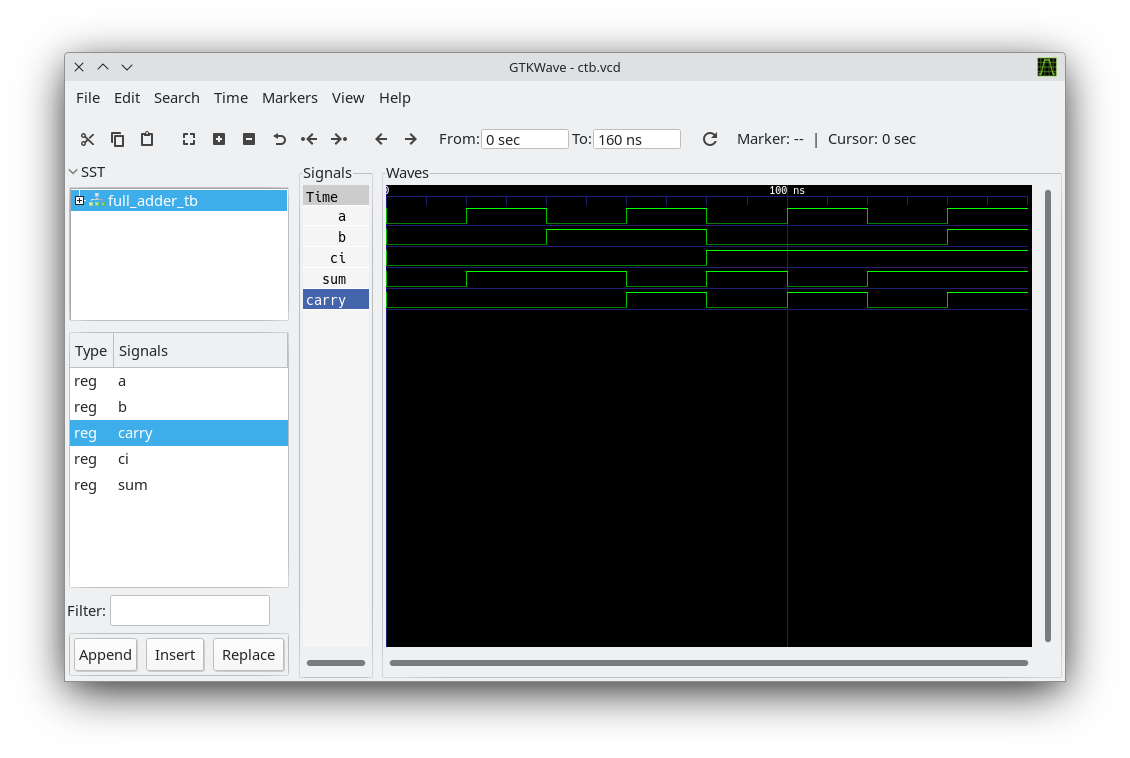
\includegraphics[width=\textwidth, height=0.5\textheight]{ctb}
\end{center}

\subsubsection{Explanation}
In the \texttt{UUT} entity of the test bench, we first use the full adder that we wrote, and then concurrently, we pass the commented truth table to the inputs of the full adder, the desired output should exists on the GTKWave output, in which it is.

\newpage
\section{Process Based Test Bench Source Code}
\begin{lstlisting}
library ieee;
use ieee.std_logic_1164.all;

entity full_adder_process_tb is
end full_adder_process_tb;

architecture tb of full_adder_process_tb is
    signal a, b, ci : std_logic;  -- inputs
    signal sum, carry : std_logic;  -- outputs
begin
-- connecting testbench signals with full_adder.vhdl
    UUT : entity work.full_adder port map (a => a, b => b, ci => ci, s => sum, c => carry);
    tb1 : process
    constant period: time := 20 ns;
        begin
            -- a b  s c
            -- 0 0  0 0
            -- 0 1  1 0
            -- 1 0  1 0
            -- 1 1  0 1

            a <= '0';
            b <= '0';
            ci <= '0';
            wait for period;
            assert ((sum = '0') and (carry = '0'))  -- expected output
            -- error will be reported if sum or carry is not 0
            report "test failed for input combination" severity error;

            a <= '0';
            b <= '1';
            ci <= '0';
            wait for period;
            assert ((sum = '1') and (carry = '0'))
            report "test failed for input combination 001" severity error;

            a <= '1';
            b <= '0';
            ci <= '0';
            wait for period;
            assert ((sum = '1') and (carry = '0'))
            report "test failed for input combination 010" severity error;

            a <= '1';
            b <= '1';
            ci <= '0';
            wait for period;
            assert ((sum = '0') and (carry = '1'))
            report "test failed for input combination 011" severity error;


            a <= '0';
            b <= '0';
            ci <= '1';
            wait for period;
            assert ((sum = '1') and (carry = '0'))  -- expected output
            -- error will be reported if sum or carry is not 0
            report "test failed for input combination 100" severity error;

            a <= '0';
            b <= '1';
            ci <= '1';
            wait for period;
            assert ((sum = '0') and (carry = '1'))
            report "test failed for input combination 101" severity error;

            a <= '1';
            b <= '0';
            ci <= '1';
            wait for period;
            assert ((sum = '0') and (carry = '1'))
            report "test failed for input combination 110" severity error;
            
            a <= '1';
            b <= '1';
            ci <= '1';
            wait for period;
            assert ((sum = '1') and (carry = '1'))
            report "test failed for input combination 111" severity error;
            
            
            assert false report "all tests passed." severity note;
            wait; -- indefinitely suspend process
    end process;
end tb ;
\end{lstlisting}
\subsection{Output Signals}
\subsubsection{Compilation Output}
\begin{center}
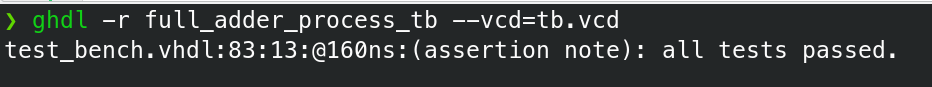
\includegraphics[width=\textwidth]{cctb}
\end{center}
\subsubsection{GTKWave Output}
\begin{center}
    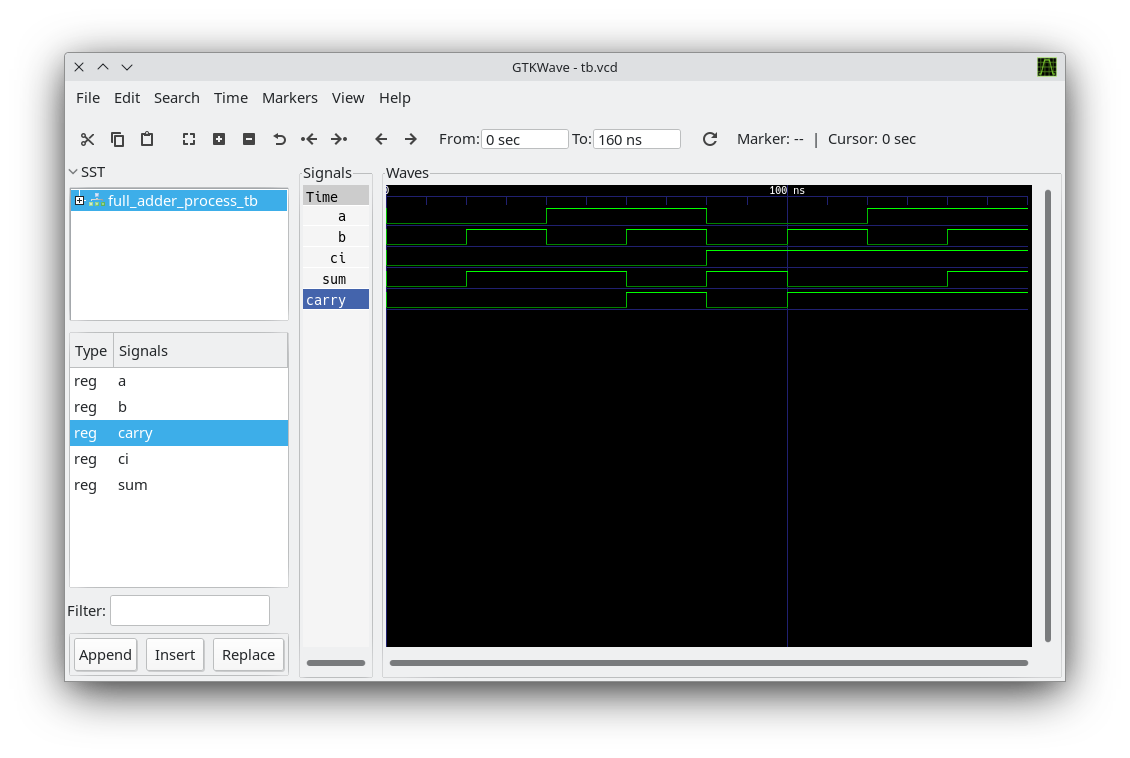
\includegraphics[width=0.8\textwidth, height=0.4\textheight]{tb}
\end{center}

\subsubsection{Explanation}
Process-based testing is another approach of writing \texttt{VHDL} test bench.

After instantiating the full adder that we wrote, we create a process named \texttt{tb1}. With the period of \texttt{20 ns} which is defined as \texttt{constant}, we pass eight diffrent inputs to the full adder.

Then, with the \texttt{assert} statement, we test the output to be desired and corrent output.
if it is not, we report a detailed message for the \textit{test case}. If all the test cases pass, we report \texttt{all tests passed.}.

This kind of testing is a little bit harder to write but has the advantage of reporting error message for the written test cases.
\end{document}